% Intended LaTeX compiler: pdflatex
\documentclass[11pt]{article}

\usepackage[utf8]{inputenc}
\usepackage[T1]{fontenc}
\usepackage{graphicx}
\usepackage{longtable}
\usepackage{wrapfig}
\usepackage{rotating}
\usepackage[normalem]{ulem}
\usepackage{amsmath}
\usepackage{amssymb}
\usepackage{capt-of}
\usepackage{hyperref}
\author{Presented by: Michael Raba for AS 390}
\date{\today}
\title{Seiga [清雅] The Architecture of Refinement\\\medskip
\large The Work of Living National Treasure Kenji Suda [須田賢司]}
\hypersetup{
 pdfauthor={Presented by: Michael Raba for AS 390},
 pdftitle={Seiga [清雅] The Architecture of Refinement},
 pdfkeywords={},
 pdfsubject={},
 pdfcreator={},
 pdflang={English}}
\begin{document}

\maketitle
\section*{Kenji Suda: The Living National Treasure (Japan)}
\label{introduction}
\subsection*{Kenji in workshop}
\label{sec:org12025cb}

\begin{center}
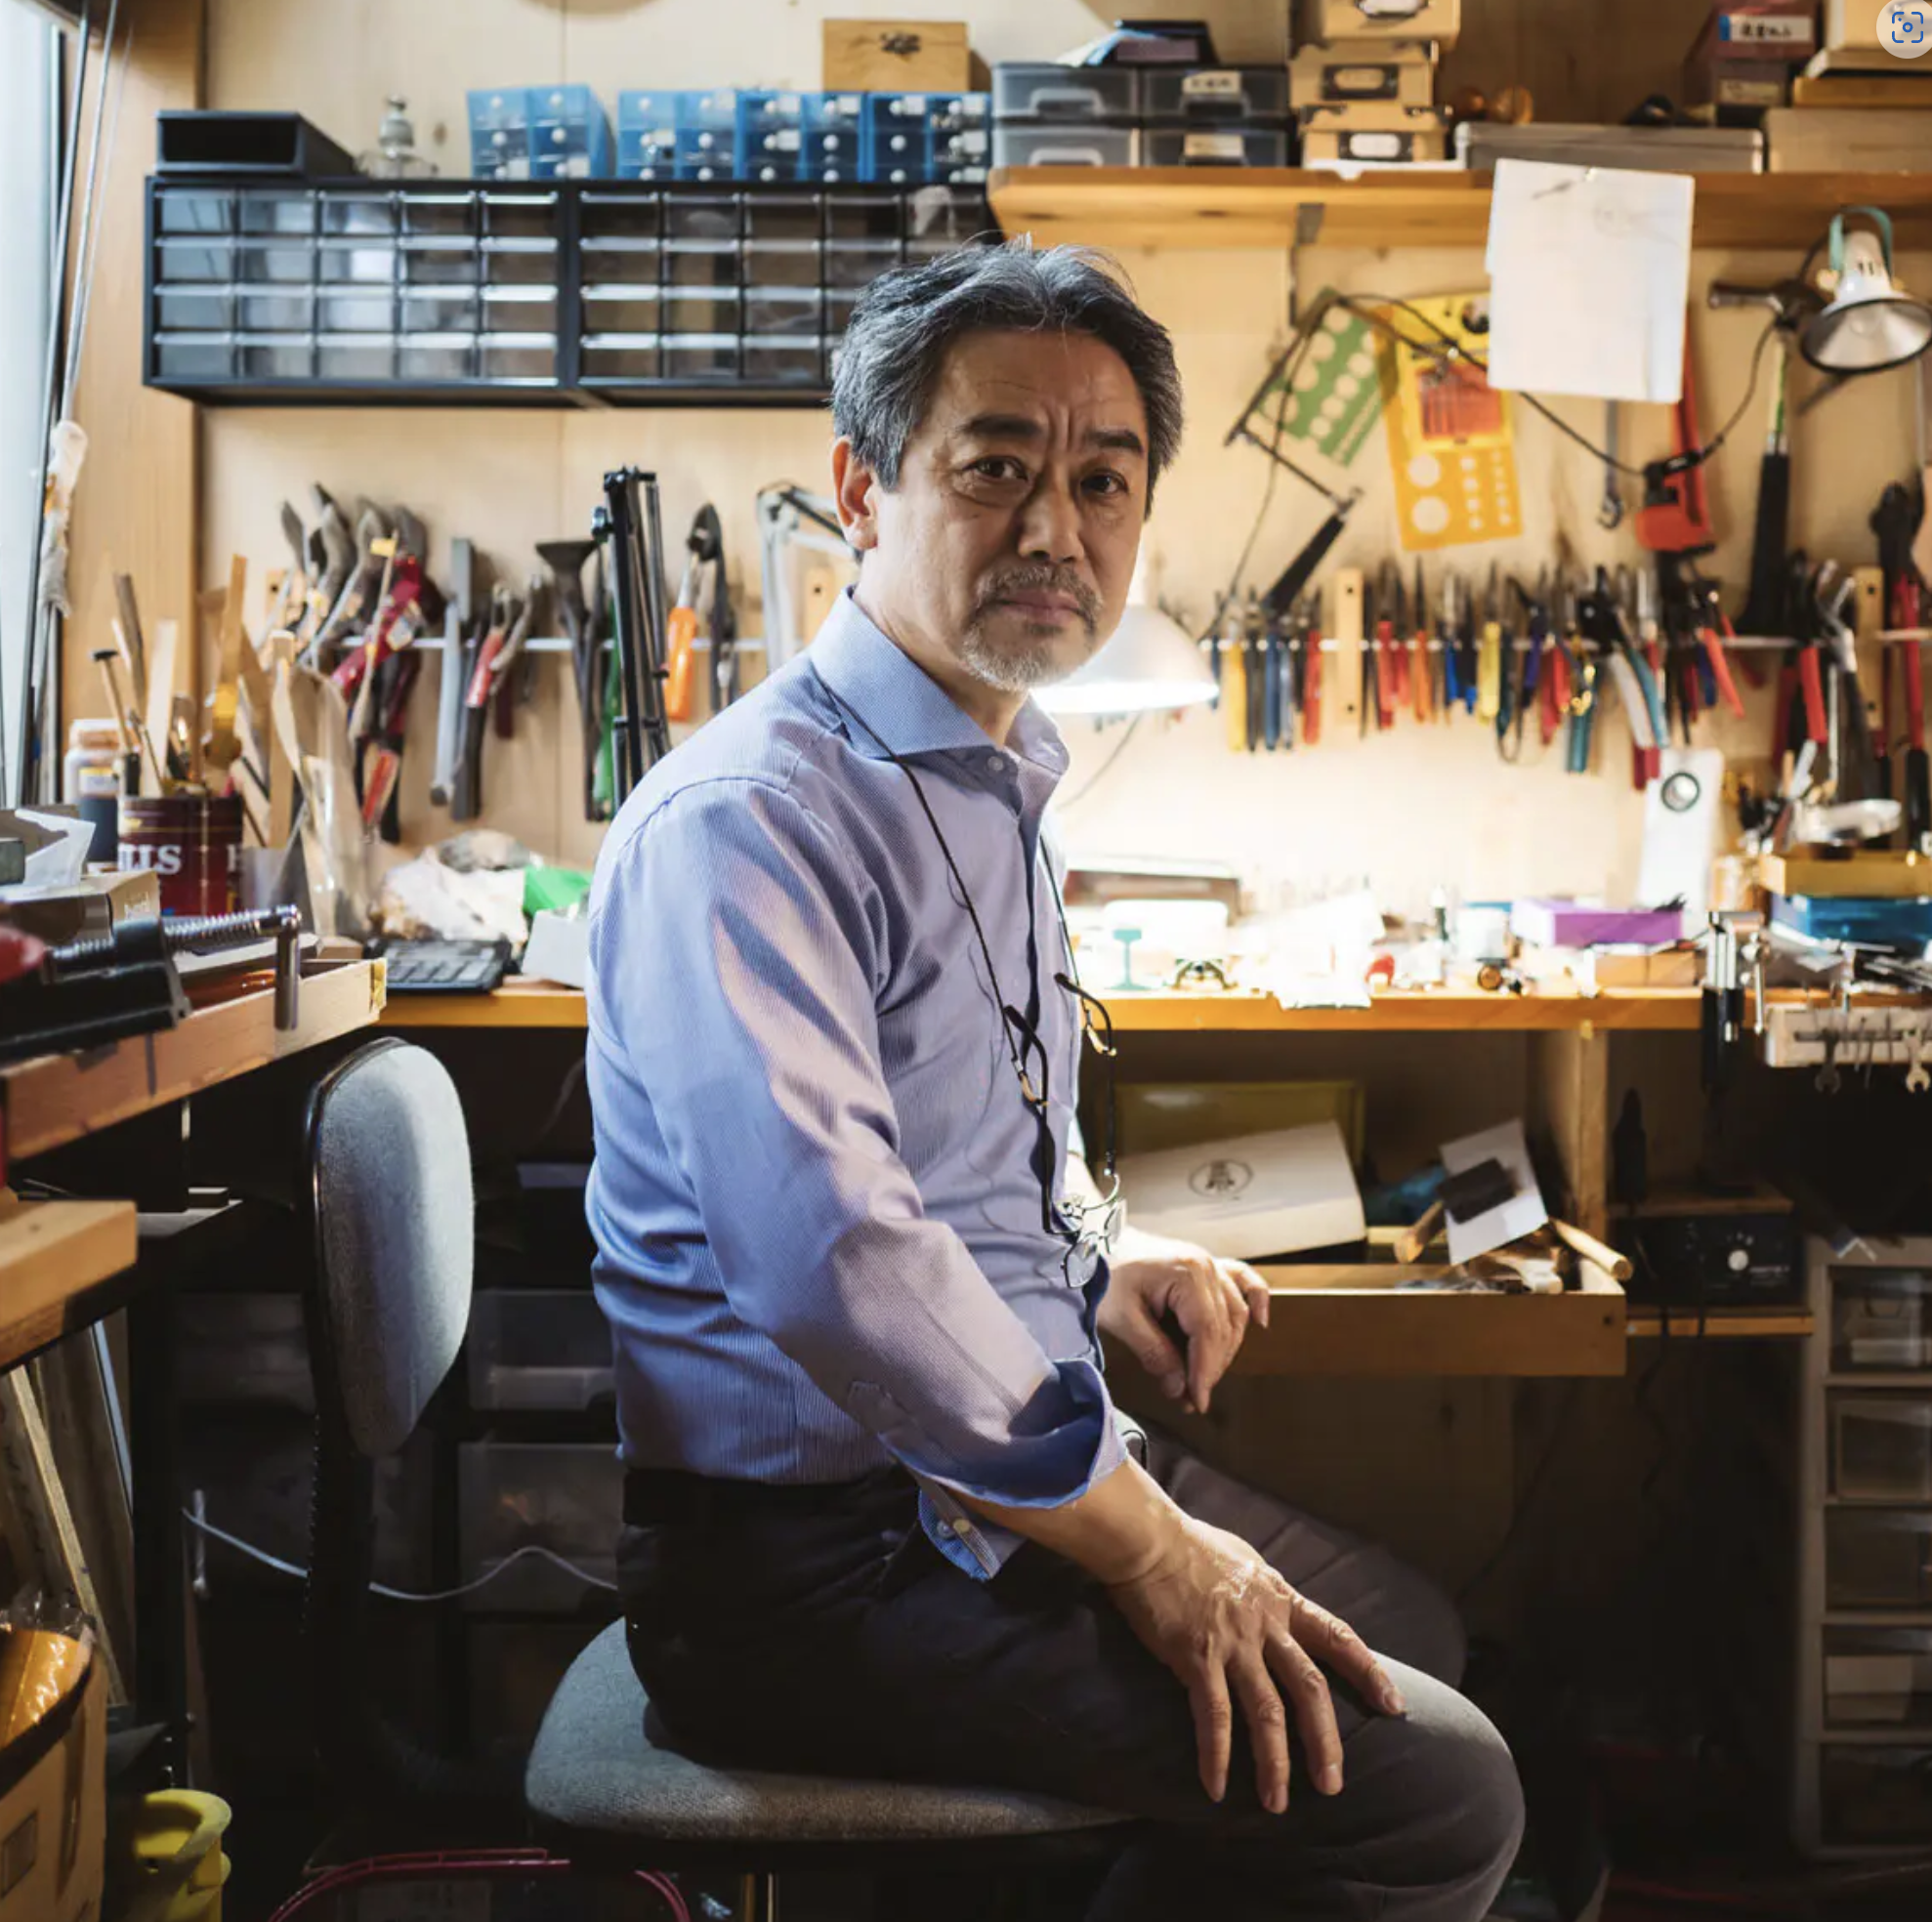
\includegraphics[width=.9\linewidth]{./images/kenji2.png}
\end{center}
\section*{Style/Technique}
\label{sec:org32d69cf}

\begin{itemize}
\item use of local kiln dried woods (mulberry)
\item unites: blacksmithing, joinery, and lacquer (fuku-urshi)
\end{itemize}
\section*{Grandfather's Plane}
\label{sec:org9b0948f}

\begin{center}
\includegraphics[width=.9\linewidth]{./images/plane.png}
\end{center}
\subsection*{Detail}
\label{sec:org123561c}

The small planes in the hand of Kenji
Suda were used by his grandfather Sogetsu, and the blades are said to be the
works of famous bladesmith Nobuyoshi. Kenji wrote that, “There is nothing more
to say except that they cut well.” The well-used tools have a particular
beauty.
\section*{Grandfather's Box}
\label{sec:org2fbbcf9}
Mulberry writing box
Creator: Suda Sogetsu (1877-1950)

\begin{center}
\includegraphics[width=.9\linewidth]{./images/grandfatherMulberry.png}
\end{center}
\subsection*{Detail}
\label{sec:orgdb33a72}

credited with elevating the family's technical standards to the elite levels required for Imperial-grade furnishings.

\begin{itemize}
\item \textbf{Imperial Household Agency} : functional, ultra-high-end furnishings meant for the environments where the Imperial family lived or held audiences.
\end{itemize}
\section*{Father's Box}
\label{sec:orgbe6079e}
Suda Kuwasui ``Black Persimmon Chest of Drawers'' 1979

\begin{center}
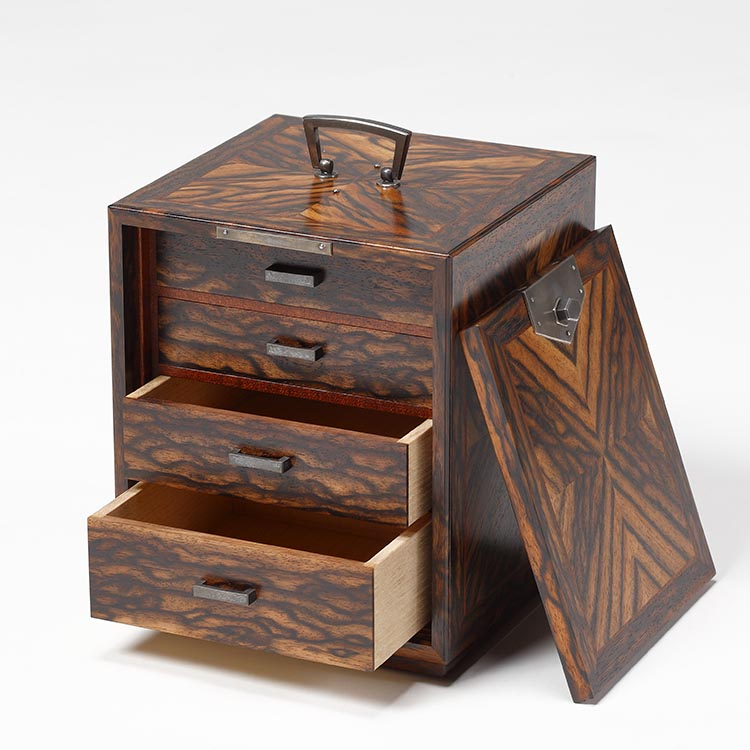
\includegraphics[width=.9\linewidth]{./images/sosui.jpg}
\end{center}
\subsection*{Detail}
\label{sec:org5d74cf5}

\begin{itemize}
\item clean lines, structural balance, and the functional beauty of the Sashimono joints.

\item National Art Exhibitions
\end{itemize}
\section*{Father's Box 2}
\label{sec:org3959db0}

\begin{center}
\includegraphics[width=.9\linewidth]{./images/fatherBox2.png}
\end{center}
\section*{Historical First}
\label{sec:orgfcfdd6a}

\begin{center}
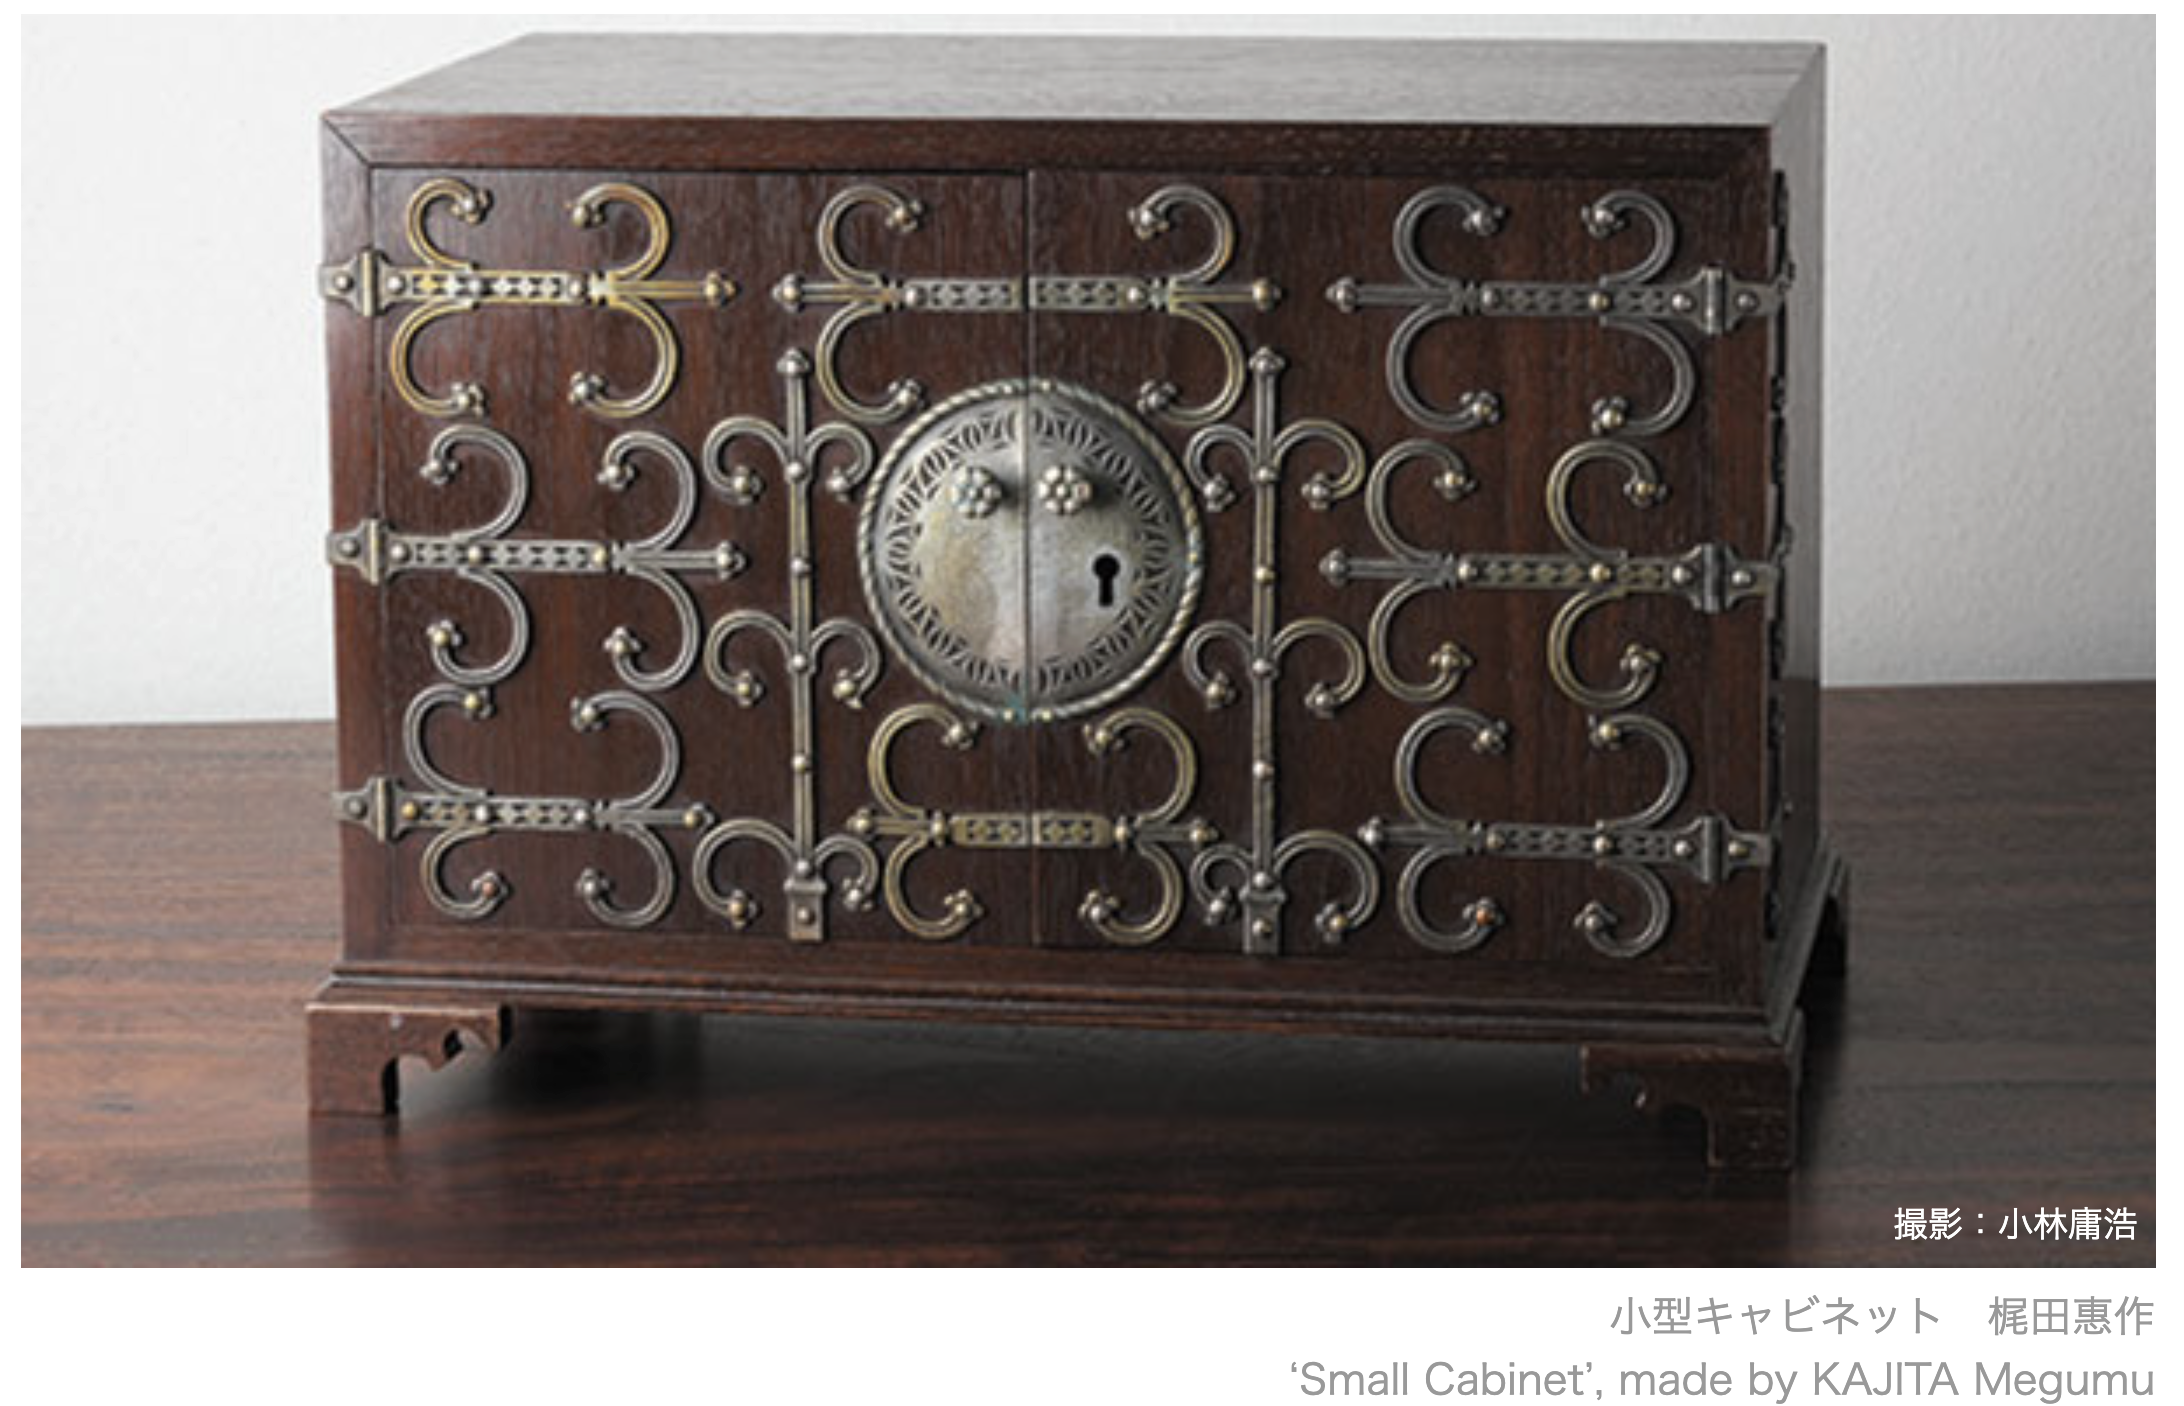
\includegraphics[width=.9\linewidth]{./images/hist1.png}
\end{center}
\subsection*{Detail}
\label{sec:org2e54200}

\begin{center}
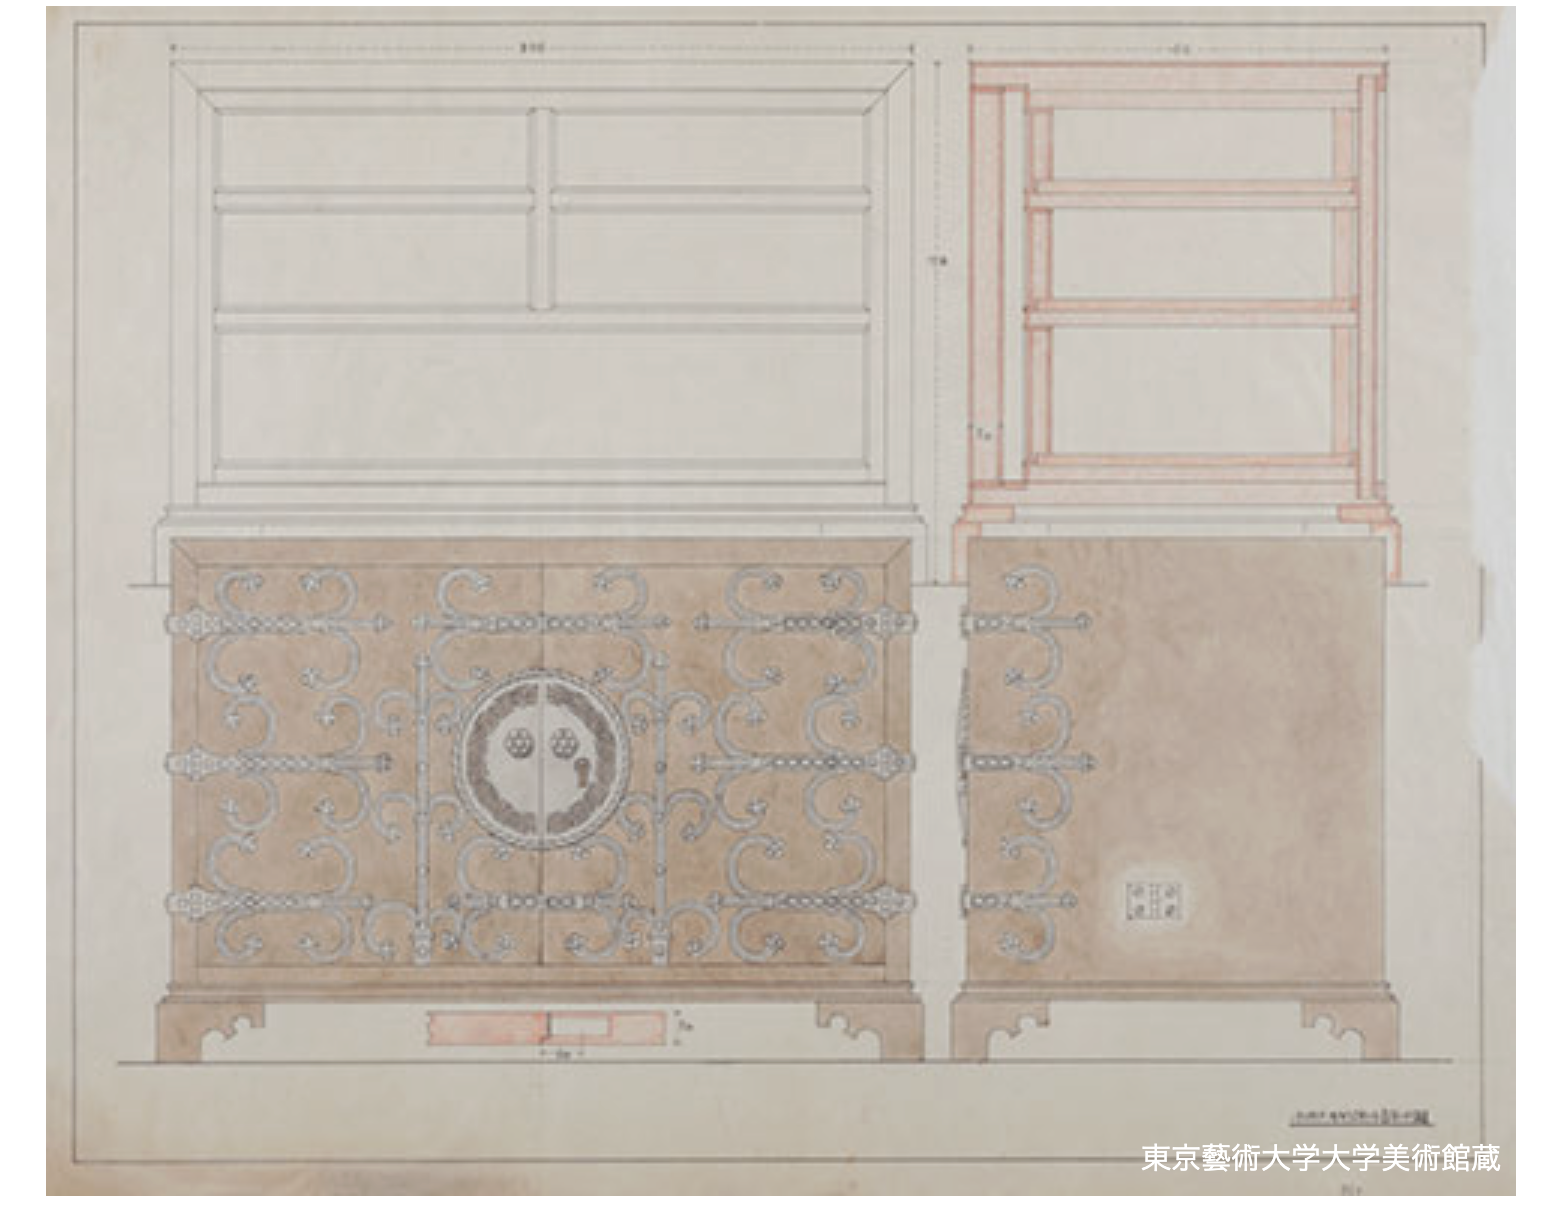
\includegraphics[width=.9\linewidth]{./images/hist2.png}
\end{center}
\subsection*{Detail}
\label{sec:orgc28efc3}

\begin{center}
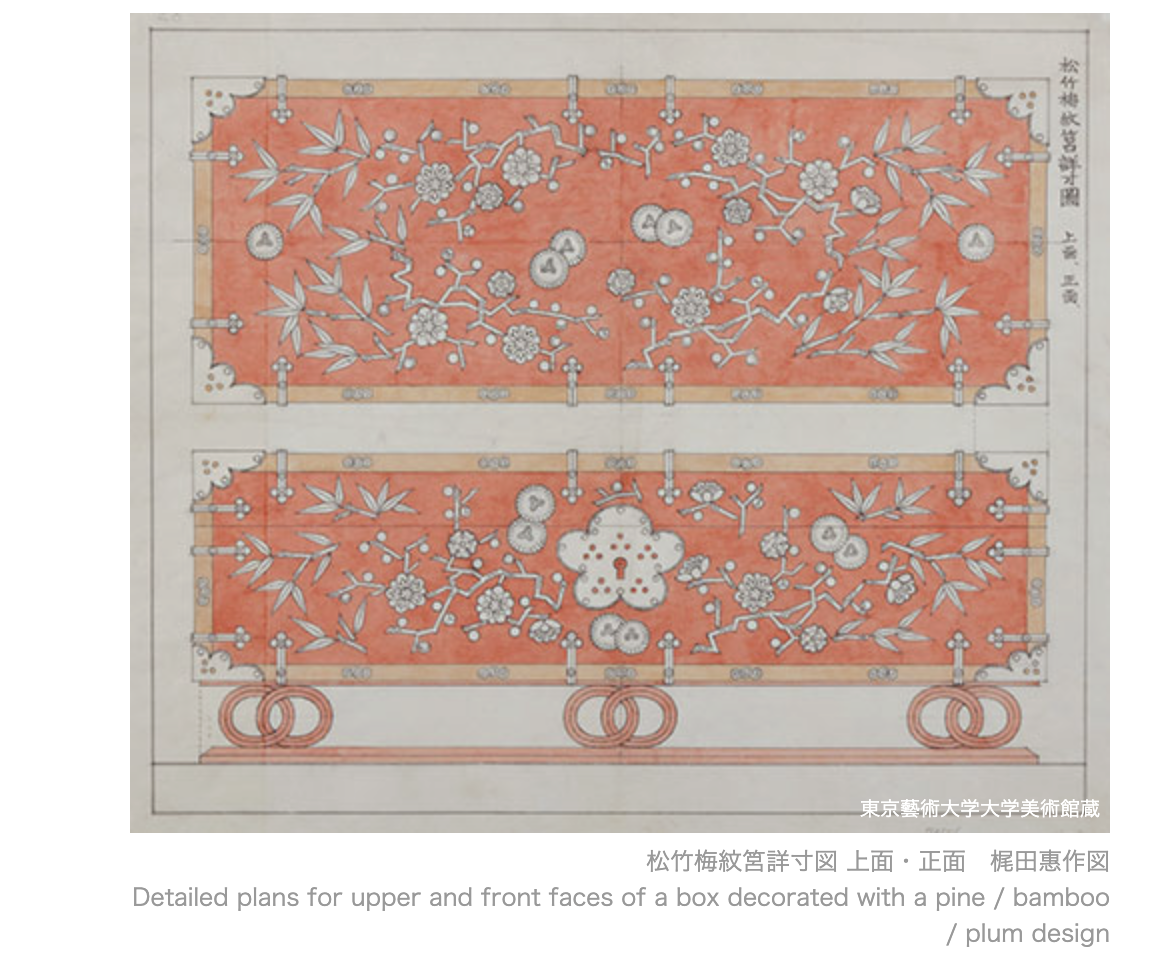
\includegraphics[width=.9\linewidth]{./images/hist3.png}
\end{center}
\section*{Suiko Box}
\label{sec:org76beaeb}


\begin{center}
\includegraphics[width=.9\linewidth]{./images/suiko.png}
\end{center}
\section*{Tsukuhae Box}
\label{sec:org197da49}
Hirin gen'ei 碑林玄英 (Stela Forest in Winter)
2013

\begin{center}
\includegraphics[width=.9\linewidth]{./images/tsu.png}
\end{center}
\subsection*{Tsukuhae Box}
\label{sec:org86c15d2}

\begin{center}
\includegraphics[width=.9\linewidth]{./images/tsu2.png}
\end{center}
\section*{Contrast}
\label{sec:org0f452a8}

Suiko captures the fluid, rhythmic energy of daylight reflecting off rippling water,

whereas Tsukuhae emphasizes the quiet, singular stillness of moonlight in the dark.

Visually, this creates a tension between the Suiko's edge-to-edge movement and the Tsukuhae's minimalist, atmospheric focus.
\section*{Joinery (Deconstructed)}
\label{sec:org826e3ac}

\begin{center}
\includegraphics[width=.9\linewidth]{./images/joinery1.png}
\end{center}
\section*{Small Box of Zelkova Finished in Wiped Urushi (2022).}
\label{sec:org5ef8fb4}

\begin{center}
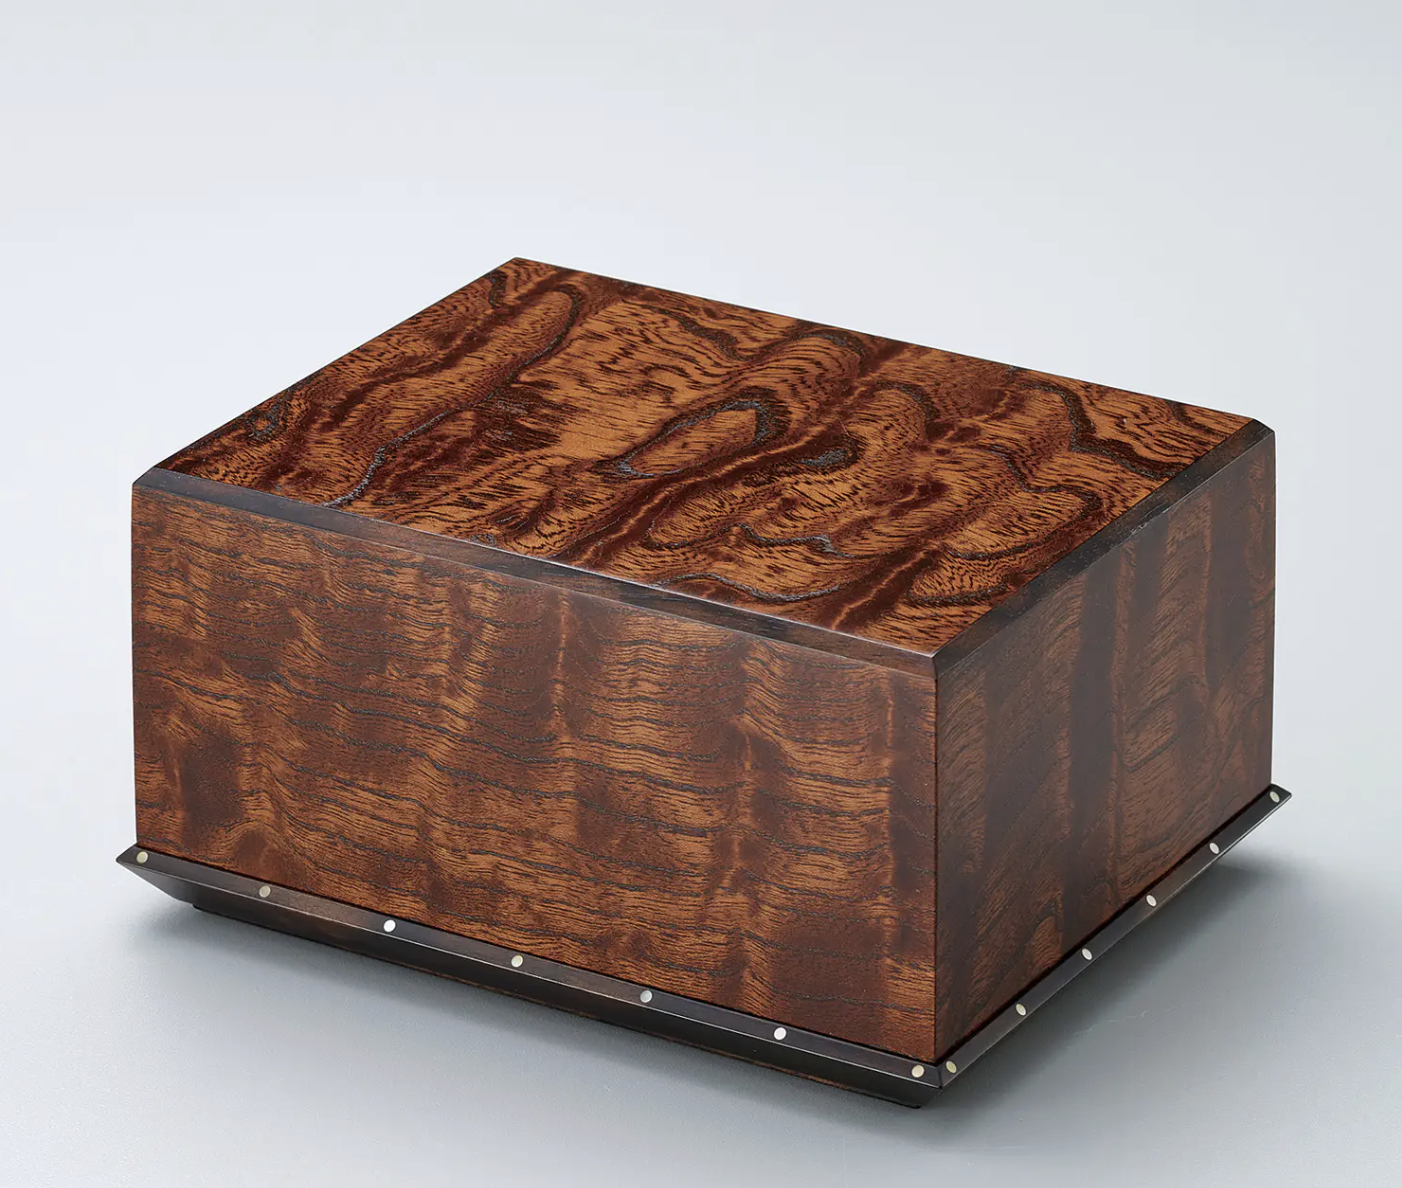
\includegraphics[width=.9\linewidth]{./images/z.png}
\end{center}
\subsection*{Analysis}
\label{sec:orgd70dc2b}

\begin{itemize}
\item Zelkova is famous for its bold, ``mountains and rivers'' grain. In this piece, Suda has selected a cut where the grain lines are broad and stable.

\item He is letting the simple, natural growth rings of the Zelkova tree do the talking, rather than relying on a flashy, ``busy'' grain to impress the viewer.
\end{itemize}
\section*{Ohotera: Table of Pear and Locust (2024)}
\label{slide-t1-intro}
\subsection*{Concept, Structure \& Materiality}
\label{slide-t1-technical}
\begin{itemize}
\item \textbf{\textbf{Concept:}} Organizing rectilinear planes with a ``Seiga'' (refined purity) motif. The formal elements emphasize horizontal massing, where the ``S-curve'' of the leg-to-apron transition creates a fluid line from the ground to the surface.
\item \textbf{\textbf{Structure:}} A \textbf{\textbf{codependent}} structural system. The table utilizes traditional \textbf{Sashimono} (blind joinery) to handle the tension of the cantilevered top. The relationship between the low height (32cm) and the wide span (114cm) requires high-precision compression joints to prevent racking without metal hardware.
\item \textbf{\textbf{Materials:}} Deploys \textbf{\textbf{Kenponashi}} (Japanese Raisin Tree/Pear) for its refined grain and \textbf{\textbf{Enju}} (Japanese Pagoda/Locust) for structural density. These choices balance the aesthetic need for ``shimmer'' with the functional requirement of a load-bearing surface.
\end{itemize}
\subsection*{Process, Details \& Context}
\label{slide-t1-context}
\section*{Sycamore Maple Box (2019)}
\label{slide-1}
\begin{center}
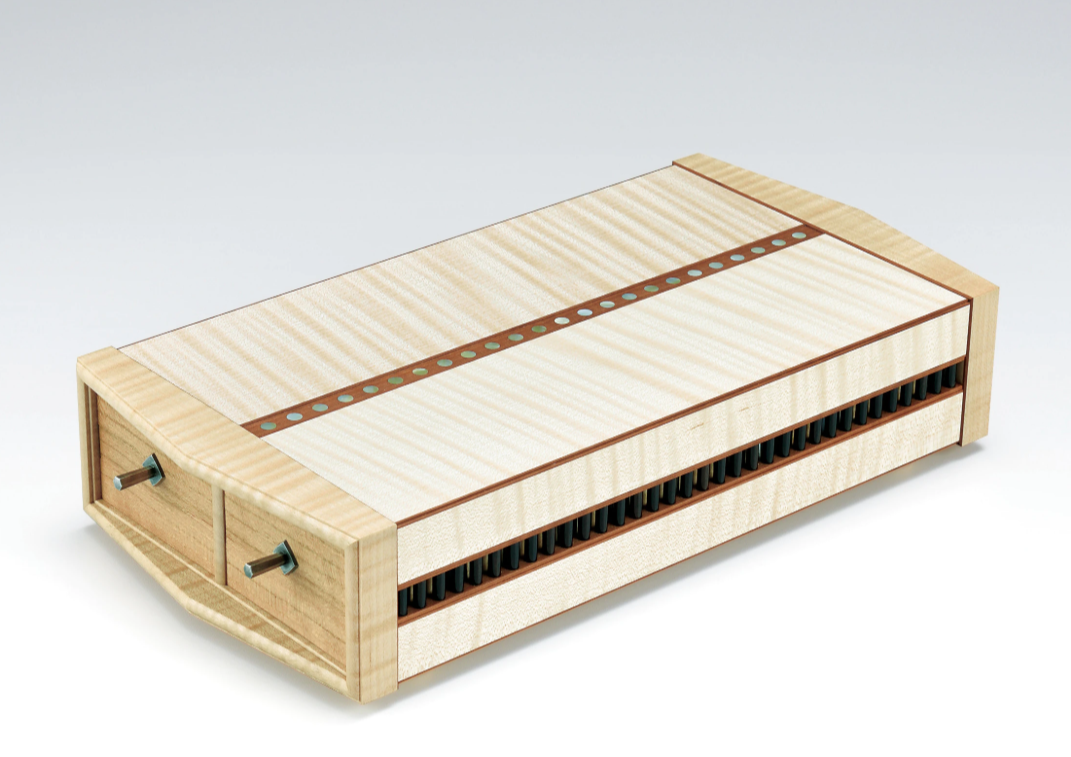
\includegraphics[width=.9\linewidth]{./images/d1.png}
\end{center}

\begin{itemize}
\item \textbf{Artisan:} Carpenter (Sashimono Specialist)
\item \textbf{Material:} Curly Maple (Sycamore)
\item \textbf{Exhibition:} 66th Japan Traditional Crafts (2019)
\end{itemize}
\subsection*{Concept, Structure \& Materiality}
\label{slide-2}
\begin{itemize}
\item \textbf{Concept:} Formal organization of rectilinear planes and rhythmic repetition; grain ``chatoyancy'' contrasts with dark vertical massing.
\item \textbf{Structure:} Codependent \textbf{Sashimono} (blind joinery) system; relies on precision-fit compression and mechanical locking without fasteners.
\item \textbf{Materials:} Curly Maple selected for aesthetic shimmer and high structural density; technology of the hand expressed through grain-matching.
\end{itemize}
\subsection*{Process, Details \& Context}
\label{slide-3}
\begin{itemize}
\item \textbf{Process:} Sequential interlocking of \textbf{tsugite} joints; fabrication is elevated to an aesthetic by exposing joinery as a serrated decorative element.
\item \textbf{Details:} Large maple chassis; Medium rhythmic joinery ``teeth''; Small metal pins and circular surface inlays.
\item \textbf{Context:} Functional sculpture for institutional/collector environments; labor-intensive fabrication justifies high-end retail price point.
\end{itemize}
\section*{Yatsuhashi II: Claro Walnut and Cherry Wood Table}
\label{slide-1}
\begin{center}
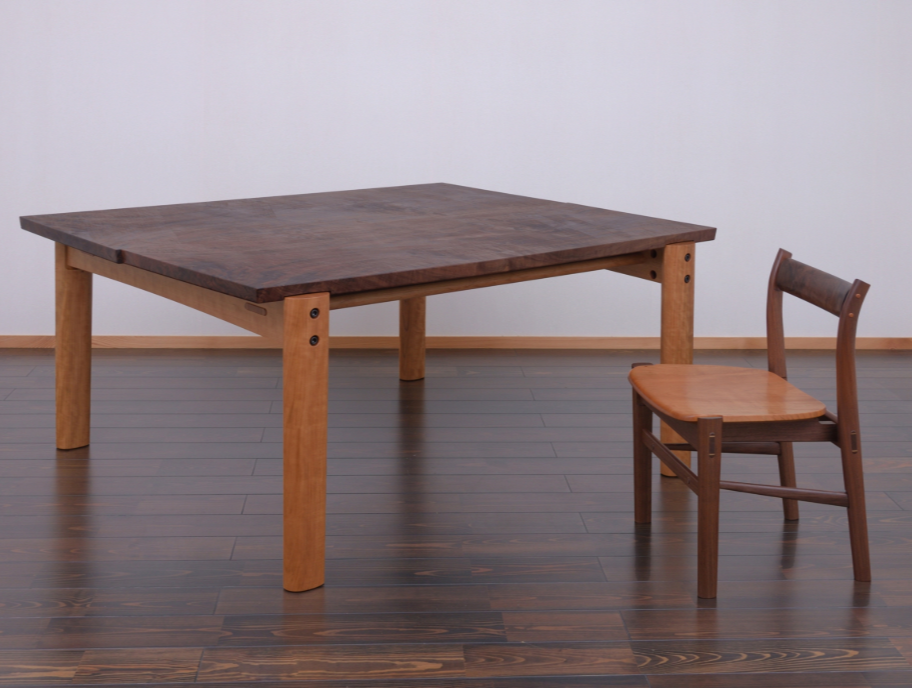
\includegraphics[width=.9\linewidth]{./images/d2.png}
\end{center}

\begin{itemize}
\item \textbf{Artisan:} Kenji Suda (Living National Treasure)
\item \textbf{Material:} Claro Walnut and Cherry Wood
\item \textbf{Dimensions:} H 72.0 x W 160.0 x D 135.0 cm
\end{itemize}
\subsection*{Concept, Structure \& Materiality}
\label{slide-2}
\subsection*{Process, Details \& Context}
\label{slide-3}
\begin{itemize}
\item \textbf{Process:} Fabricated using high-precision \textbf{Sashimono} (wood joinery) and finished in wiped lacquer (\textbf{urushi}) to accentuate the grain without masking the tactile surface.
\item \textbf{Details:} Large interlocking walnut planks; Medium cherry structural beams; Small precisely carved joint interfaces where the ``planks'' meet the frame.
\item \textbf{Context:} A monumental functional sculpture intended for institutional or high-end residential interiors; its status as a work by a Living National Treasure places it in a high-luxury price bracket for serious collectors.
\end{itemize}
\section*{Philosophy: Craft as Life [生活 - Seikatsu]}
\label{philosophy}
\end{document}
